% ============================================================
%  SECTION 2: The foreign exchange market        (Member 1)
% ============================================================
\section{The foreign exchange market: who needs dollars and who supplies them?}\label{sec:forex}

Currencies are bought and sold in the \keyterm{foreign exchange market}{The market in which currencies are traded for one another. Also called the forex market.}, or forex market. It has no building and no closing bell. It is a worldwide network of banks, dealers and large firms that trade with each other electronically, and as the day moves from Tokyo and Singapore to Mumbai, London and New York, the trading moves with it (Greenlaw et al., 2022).

Figure~\ref{fig:m1-flow} sorts the people in this market into two groups. Importers, students and travellers abroad, Indians investing abroad and anyone repaying a foreign loan need dollars. Together they make up the \keyterm{demand for foreign exchange}{The foreign currency that residents want, to pay for imports, study and travel abroad, investment abroad and foreign loans.}. Exporters like Selvi, whose garment unit in Tiruppur sells T-shirts to American shops, workers abroad like Ravi who send home \keyterm{remittances}{Money that people working abroad send home to their families.}, foreign tourists and foreign investors all bring dollars in. They make up the \keyterm{supply of foreign exchange}{The foreign currency flowing into a country from its exports, remittances, tourists and foreign investment.} (NCERT, 2007). Every deal is two purchases at once: when Meera's father buys dollars, he is also selling rupees (Greenlaw et al., 2022). The exchange rate is the price at which the two sides match \seesec{sec:ds}.

\begin{figure}[!htb]
  \centering
  \resizebox{\linewidth}{!}{% Figure M1-2: who demands and who supplies US dollars in India's forex market.
% Drawn in TikZ so it stays sharp and editable. Uses colours from fxstyle.sty.
\begin{tikzpicture}[
  font=\sffamily\small, every node/.append style={execute at begin node={\spaceskip=0.24em plus 0.04em minus 0.02em\relax}},
  item/.style={draw=none, fill=white, rounded corners=1.2mm, minimum height=9.2mm,
               text width=48mm, align=left, execute at begin node={\hyphenpenalty=10000\relax}, inner xsep=7pt, inner ysep=3pt},
  head/.style={text=white, font=\sffamily\bfseries, align=center, text width=52mm,
               minimum height=12mm, rounded corners=1.5mm},
  who/.style={font=\sffamily\scriptsize\itshape, text=fxmuted},
  flow/.style={-{Stealth[length=3.2mm,width=2.6mm]}, line width=1.6pt},
]
% ---- left column: demand ----
\node[head, fill=fxorange] (dh) at (0,0)
  {Who wants dollars?\\[-1pt]{\footnotesize\mdseries demand for foreign exchange}};
\node[item, below=3mm of dh] (d1) {\textbf{Importers}\\[-1pt]{\footnotesize crude oil, gold, electronics, machines}};
\node[item, below=2mm of d1] (d2) {\textbf{Students and travellers abroad}\\[-1pt]{\footnotesize \textcolor{fxorange}{e.g.\ Meera's college fees}}};
\node[item, below=2mm of d2] (d3) {\textbf{Indians investing abroad}\\[-1pt]{\footnotesize shares, property, firms}};
\node[item, below=2mm of d3] (d4) {\textbf{Repaying foreign loans}\\[-1pt]{\footnotesize firms and government}};
\begin{scope}[on background layer]
  \node[fill=fxorange!10, rounded corners=2mm, inner sep=3mm, fit=(dh)(d4)] (dbox) {};
\end{scope}

% ---- right column: supply ----
\node[head, fill=fxteal] (sh) at (13.4,0)
  {Who brings dollars in?\\[-1pt]{\footnotesize\mdseries supply of foreign exchange}};
\node[item, below=3mm of sh] (s1) {\textbf{Exporters}\\[-1pt]{\footnotesize \textcolor{fxteal}{e.g.\ Selvi's T-shirts}, IT services}};
\node[item, below=2mm of s1] (s2) {\textbf{Remittances}\\[-1pt]{\footnotesize \textcolor{fxteal}{e.g.\ Ravi's money from Dubai}}};
\node[item, below=2mm of s2] (s3) {\textbf{Foreign tourists in India}\\[-1pt]{\footnotesize hotels, travel, shopping}};
\node[item, below=2mm of s3] (s4) {\textbf{Foreigners investing in India}\\[-1pt]{\footnotesize FDI and FPI}};
\begin{scope}[on background layer]
  \node[fill=fxteal!10, rounded corners=2mm, inner sep=3mm, fit=(sh)(s4)] (sbox) {};
\end{scope}

% ---- centre: the market ----
\coordinate (mid) at ($(dbox.east)!0.5!(sbox.west)$);
\node[fill=fxnavy, text=white, rounded corners=3mm, text width=36mm, align=center,
      minimum height=34mm, inner sep=6pt] (mkt) at (mid)
  {\heavysans\large Foreign\\exchange market\\[5pt]
   {\footnotesize\sffamily banks and other authorised dealers, regulated by the RBI}};
\node[fill=white, draw=fxnavy, line width=0.8pt, rounded corners=1.5mm, below=4mm of mkt,
      align=center, text width=34mm, inner sep=4pt] (price)
  {{\footnotesize\color{fxmuted}the price that clears it}\\[-1pt]{\heavysans\color{fxnavy}\large ₹ per US dollar}};

% ---- flows ----
\draw[flow, fxorange] (dbox.east |- mkt.150) -- (mkt.150)
  node[pos=0.5, above=1pt, font=\sffamily\scriptsize\bfseries, text=fxorange, align=center] {offer rupees,\\ want dollars};
\draw[flow, fxteal] (sbox.west |- mkt.30) -- (mkt.30)
  node[pos=0.5, above=1pt, font=\sffamily\scriptsize\bfseries, text=fxteal, align=center] {offer dollars,\\ want rupees};
\end{tikzpicture}
}
  \caption{Who wants dollars and who brings them in.}
  \label{fig:m1-flow}
  {\raggedright\small\sffamily Each group on the left offers rupees to get dollars. Each group on the right offers dollars to get rupees.\par}
  \figsource{Drawn by the authors, based on NCERT (2007, Chapter 6) and Greenlaw et al. (2022, Section 29.1).}
\end{figure}

\subsection{Most currency trading is not about trade}
In April 2025, about US\$9.6 trillion worth of currencies changed hands every day (BIS, 2025). All the world's exports of goods and services in 2024 were worth about 33 trillion dollars (United Nations Conference on Trade and Development [UNCTAD], 2025). So the forex market trades a whole year of world exports in less than four days. Most of this trading is done by banks and investors moving savings between countries.

Investors come in two kinds. \keyterm{Foreign direct investment (FDI)}{Buying a lasting stake (10\% or more) in a business abroad, or setting one up.} buys a lasting stake in a business, like a carmaker building a factory near Chennai, and it stays for years. \keyterm{Foreign portfolio investment (FPI)}{Buying shares and bonds (holdings under 10\%), which can be sold quickly.} buys shares and bonds, and it can leave in a single day (Greenlaw et al., 2022). That is why its comings and goings can jolt the rupee \seesec{sec:moves}.

To buy dollars for the fees, Meera's father will simply walk into his bank in Chennai. Under the Foreign Exchange Management Act, 1999, only banks and firms licensed by the RBI, such as \keyterm{authorised dealers}{Banks and firms licensed by the RBI under FEMA, 1999, to buy and sell foreign currency.} and money changers, may deal in foreign currency. They trade with customers, with each other and with banks abroad, while the RBI makes the rules and, at times, buys or sells dollars itself \seesec{sec:reserves}.

\begin{casestudy}{Selvi's three-month gamble}
In October, Selvi agrees to sell T-shirts worth US\$20,000 to a shop in New York, which will pay in January. At today's rate of ₹95, that is ₹19 lakh. But if the rupee strengthens to ₹90 by January, she will receive only ₹18 lakh, and her profit could vanish. To avoid the gamble, Selvi can sign a \textbf{forward contract} with her bank today, fixing the rate at which the bank will buy her dollars in January. The rate for a deal settled today is the \textbf{spot rate}. A rate agreed today for a deal in the future is a \textbf{forward rate}. Importers use the same tool to protect themselves from a weaker rupee.
\figsource{The figures in this example are hypothetical.}
\end{casestudy}

\begin{economistsfacts}{Ravi is one of millions}
\centering
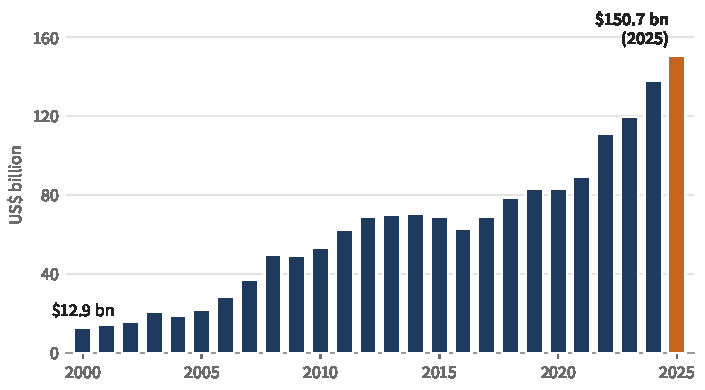
\includegraphics[width=\linewidth]{figures/remittances.pdf}
\captionof{figure}{Remittances received by India, 2000--2025 (US\$ billion).}\label{fig:m1-remit}
\figsource{World Bank (2026a), World Development Indicators, series BX.TRF.PWKR.CD.DT.}
\raggedright
In 2025, Indians working abroad sent home \textbf{US\$150.7 billion}, more than any other country received and more than twice as much as Mexico, the next-largest recipient (World Bank, 2026a). Where the money comes from is changing. In 2020-21 the US sent 23.4 per cent of it and the UAE 18.0 per cent. By 2023-24 the US share had risen to 27.7 per cent, while the UAE's had barely moved, to 19.2 per cent. An RBI study links this to more skilled Indians working in advanced economies (Gajbhiye et al., 2025).\par
\textbf{Read the chart.} (a) Roughly how many times larger were remittances in 2025 than in 2000? (b) In which year did they fall most sharply, and what might explain it?
\answers{(a) About 12 times (150.7 ÷ 12.9 ≈ 11.7). (b) 2016, when they fell about 9 per cent. The World Bank linked the fall to low oil prices and government spending cuts in the Gulf countries, where many Indians work (World Bank, 2017).}
\end{economistsfacts}

\begin{exercise}{Dollars in or dollars out?}
For each transaction, decide whether it adds to India's \emph{demand} for dollars or to the \emph{supply} of dollars.
\begin{enumerate}[label=(\alph*), leftmargin=2em]
  \item Meera's father pays her first-year fees.
  \item Ravi sends 3,000 dirhams to his parents in Thanjavur.
  \item A shop in New York pays Selvi for 5,000 T-shirts.
  \item A Japanese carmaker builds a new factory in Tamil Nadu.
  \item An Indian oil company buys a shipload of crude oil.
  \item An American investor sells her Indian shares and takes the money home.
  \item A family from Germany spends a week on a Kerala houseboat.
\end{enumerate}
\answers{Supply: (b), (c), (d), (g). Demand: (a), (e), (f).}
\end{exercise}
% [removed at merge] Member 1's "Watch and learn" box: the same Khan Academy
% video is listed first in Further learning at the end of the chapter.
